\documentclass[11pt,a4paper]{article}
\usepackage[margin=2.2cm]{geometry}
\usepackage[T1]{fontenc}
\usepackage{lmodern}
\usepackage{microtype}
\usepackage{graphicx}
\usepackage{booktabs}
\usepackage{tabularx}
\usepackage{xcolor}
\usepackage{listings}
\usepackage{caption}
\usepackage{enumitem}
\usepackage{float}
\usepackage[hidelinks]{hyperref}

\definecolor{codebg}{HTML}{F7F7F7}
\definecolor{addline}{HTML}{1E7B34}
\definecolor{delline}{HTML}{B31D28}
\definecolor{bad}{HTML}{C0392B}
\definecolor{good}{HTML}{1F5FA8}
\captionsetup{font=small,labelfont=bf}
\setlist{itemsep=1pt,topsep=3pt}
\emergencystretch=2em
\lstset{basicstyle=\ttfamily\footnotesize, backgroundcolor=\color{codebg}, frame=single,
  rulecolor=\color{black!20}, columns=fullflexible, keepspaces=true, breaklines=true,
  showstringspaces=false, xleftmargin=3pt, xrightmargin=3pt, aboveskip=5pt, belowskip=5pt}
\lstdefinestyle{diff}{moredelim=[il][\color{addline}]{+}, moredelim=[il][\color{delline}]{-}}
\lstdefinestyle{out}{backgroundcolor=\color{black!3}}

\newcommand{\acc}{\texttt{AimdAccumulator}}
\newcommand{\aw}{\texttt{AimdWindow}}

\title{\textbf{An unsigned underflow in MsQuic's CUBIC}\\[3pt]
  \large Evidence report: the bug, a two-line fix, and why it is not our mistake}
\author{Abhiram Suresh}
\date{November 2026}

\begin{document}
\maketitle

\begin{abstract}
\noindent
In MsQuic's CUBIC congestion controller, the Reno-friendly window \aw\ is grown
\emph{before} the accumulator \acc\ is reduced by it. Both are \texttt{uint32},
so whenever an ACK carries the accumulator past the window by less than one
packet, the subtraction wraps to about $4.29\times10^9$. From then on every ACK
grows \aw\ (and, in the Reno-friendly region, the congestion window) by one
packet: CUBIC behaves like slow start in congestion avoidance. Swapping the two
lines fixes it. This report collects the evidence that the bug is real, is in
\emph{unmodified upstream} MsQuic (\texttt{main} at \texttt{3c9ec01c1},
10 November 2026), is caused by these two lines alone, and that the fix
changes nothing else. The unit-test and debugger evidence was also re-run
independently on GitHub's servers, against upstream \texttt{main} cloned
directly from GitHub. On an emulated network path, logging the accumulator
shows a wrap in all 20 upstream runs and in none of the 20 fixed runs. In plain
bulk transfers without a rate-limited phase the wrap is usually undone by the
next ACK, but it persisted in 10 of 40 upstream runs (0 of 40 fixed), and those
runs lost 5--130 times more packets than the fixed build's median. Every claim below is followed by raw output of a tool
(test runner, debugger, trace) that anyone can regenerate with the commands in
Section~\ref{sec:repro}.
\end{abstract}

\section{The bug and the fix}

\begin{lstlisting}[style=diff,title={\footnotesize\texttt{src/core/cubic.c}, \texttt{CubicCongestionControlOnDataAcknowledged} (upstream \texttt{main}, lines 659--662)}]
         if (Cubic->AimdAccumulator > Cubic->AimdWindow) {
-            Cubic->AimdWindow += DatagramPayloadLength;
             Cubic->AimdAccumulator -= Cubic->AimdWindow;
+            Cubic->AimdWindow += DatagramPayloadLength;
         }
\end{lstlisting}

\paragraph{What the code is meant to do.} The comment above it says: record
ACKed bytes in an accumulator ``until at least a window (or two windows) worth
of bytes are ACKed, and then increase the window by 1 MTU''. So when the
accumulator passes the window, one window's worth of bytes should be taken out
of it and the window grown by one packet.

\paragraph{What it does.} It grows the window first and then subtracts the
\emph{grown} window, which is one packet more than was accumulated. A worked
example with the numbers caught by the debugger in Section~\ref{sec:gdb}:
\begin{center}\small
\begin{tabular}{@{}lrr@{}}
\toprule
 & upstream order & fixed order \\
\midrule
\aw\ before & 11\,211 & 11\,211 \\
\acc\ after this ACK & 11\,704 & 11\,704 \\
\acc\ after subtracting & $11\,704 - 12\,443 \to$ \textcolor{bad}{\textbf{4\,294\,966\,557}} & $11\,704 - 11\,211 =$ \textcolor{good}{\textbf{493}} \\
\aw\ after & 12\,443 & 12\,443 \\
\bottomrule
\end{tabular}
\end{center}
With the wrapped value the condition \texttt{AimdAccumulator > AimdWindow} is
true on every following ACK, and each of them adds one packet to \aw. Because
CUBIC sets \texttt{CongestionWindow = AimdWindow} whenever \aw\ exceeds the
cubic curve, the congestion window grows by one packet per ACK, i.e.\ it
doubles every round trip, until the wrapped value has been counted down.
Congestion events reset \aw\ but not the accumulator, so the effect survives
losses.

\paragraph{Why it went unnoticed.} Three reasons, each shown below.
(1)~If the window is an exact multiple of the packet size and every ACK adds
the same amount, the next ACK wraps the accumulator straight back to a small
value and nothing visible happens; upstream's tests use such round numbers.
(2)~Two existing upstream tests \emph{do} trigger the wrap, but neither checks
the accumulator, so they pass (Section~\ref{sec:gdb}). (3)~Upstream's test
\texttt{AIMD\_\allowbreak{}Accumulator\allowbreak{}Triggers\allowbreak{}Window\allowbreak{}Growth} chooses its ACK size, in its
own words, ``to avoid unsigned underflow in the subtraction
(AimdAccumulator -= AimdWindow)''.

\paragraph{How long it has been there.} \texttt{git blame} on upstream
\texttt{main} attributes the condition and the subtraction to the CUBIC rewrite
in PR~\#2269 (\texttt{586141e1a}, January 2022), which already grew the window
first (by \texttt{Paths[0].Mtu} at the time). PR~\#2296 (\texttt{ba0819664})
changed only the amount added, to \texttt{DatagramPayloadLength}. The order is
therefore in every release since v2.0.0; it is not a recent regression.

%======================================================================
\section{Evidence 1: reproducers on unmodified upstream \texttt{main}}
\label{sec:repro1}

We checked out upstream \texttt{main} (\texttt{3c9ec01c1}, 10 Nov 2026) in a
separate worktree, with none of our other changes, and added two unit tests
to upstream's own \texttt{CubicTest.cpp} using upstream's own test fixture:
\begin{itemize}
  \item \texttt{AIMD\_AccumulatorNoUnderflow} (state level): sets up an
        accumulator 50\,B below the window and acknowledges 100\,B. The
        accumulator must then hold 50.
  \item \texttt{AIMD\_PerPacketAcksGrowAtMostOneMssPerWindow} (behaviour
        level): \emph{no internal field is set}. After one loss, the test sends
        a full window per round trip and acknowledges every packet separately,
        as a real path does, using only the public callbacks. It asserts what
        the algorithm promises: \aw\ grows by at most one packet per \aw\ bytes
        acknowledged.
\end{itemize}

\paragraph{Before the fix} (upstream \texttt{cubic.c} unchanged), verbatim:
\begin{lstlisting}[style=out]
src/core/unittest/CubicTest.cpp:2342: Failure
Expected equality of these values:
  Cubic->AimdAccumulator
    Which is: 4294966114
  50u
    Which is: 50
[  FAILED  ] CubicTest.AIMD_AccumulatorNoUnderflow (0 ms)
round 0: cwnd 11211 -> 11957, AimdWindow 11211 -> 11211, AimdAccumulator 5544
round 1: cwnd 11957 -> 12384, AimdWindow 11211 -> 11211, AimdAccumulator 11088
round 2: cwnd 12384 -> 23531, AimdWindow 11211 -> 23531, AimdAccumulator 4294808370
src/core/unittest/CubicTest.cpp:2388: Failure
Expected: (Cubic->AimdWindow - AimdBefore) <= (MaxGrowth), actual: 12320 vs 2464
[  FAILED  ] CubicTest.AIMD_PerPacketAcksGrowAtMostOneMssPerWindow (0 ms)
\end{lstlisting}
In round 2 the congestion window goes from 12\,384 to 23\,531 bytes in one
round trip of congestion avoidance (+90\,\%), and \aw\ grows by ten packets
where two is the maximum.

\paragraph{After swapping the two lines} (nothing else in \texttt{cubic.c} changed):
\begin{lstlisting}[style=out]
[       OK ] CubicTest.AIMD_AccumulatorNoUnderflow (0 ms)
round 0: cwnd 11211 -> 11957, AimdWindow 11211 -> 11211, AimdAccumulator 5544
round 1: cwnd 11957 -> 12384, AimdWindow 11211 -> 11211, AimdAccumulator 11088
round 2: cwnd 12384 -> 12716, AimdWindow 11211 -> 12443, AimdAccumulator 6037
round 3: cwnd 12716 -> 12985, AimdWindow 12443 -> 12443, AimdAccumulator 12197
round 4: cwnd 12985 -> 13675, AimdWindow 12443 -> 13675, AimdAccumulator 5914
round 5: cwnd 13675 -> 13675, AimdWindow 13675 -> 13675, AimdAccumulator 12690
round 6: cwnd 13675 -> 14907, AimdWindow 13675 -> 14907, AimdAccumulator 5791
round 7: cwnd 14907 -> 14907, AimdWindow 14907 -> 14907, AimdAccumulator 13183
[       OK ] CubicTest.AIMD_PerPacketAcksGrowAtMostOneMssPerWindow (0 ms)
\end{lstlisting}
Rounds 0--1 are identical in both runs: the two versions only differ from the
moment the accumulator crosses the window.

%======================================================================
\section{Evidence 2: a debugger catches the wrap in upstream code}
\label{sec:gdb}

To take our own code out of the picture entirely, we let \texttt{gdb} watch
upstream's unmodified \texttt{cubic.c}. A breakpoint on line 661
(\texttt{AimdAccumulator -= AimdWindow}) fires only if the subtraction is
about to go below zero, prints both operands and the \texttt{uint32} result,
and records which test is running. Run over \emph{upstream's own, unmodified}
\texttt{CubicTest} suite:
\begin{lstlisting}[style=out]
[ RUN      ] CubicTest.CongestionAvoidance_BoundedGrowthClamp
=== underflow 1 at cubic.c:661  AimdAccumulator -= AimdWindow ===
AimdWindow (already grown on line 660) = 1232
AimdAccumulator before the subtraction = 1200
AimdAccumulator after (uint32 result)  = 4294967264
#1  CubicTest_CongestionAvoidance_BoundedGrowthClamp_Test::TestBody at src/core/unittest/CubicTest.cpp:761
[       OK ] CubicTest.CongestionAvoidance_BoundedGrowthClamp (1 ms)
...
[ RUN      ] CubicTest.CongestionAvoidance_TimeGapOverflowProtection
=== underflow 2 at cubic.c:661  AimdAccumulator -= AimdWindow ===
AimdWindow (already grown on line 660) = 1232
AimdAccumulator before the subtraction = 1200
AimdAccumulator after (uint32 result)  = 4294967264
#1  CubicTest_CongestionAvoidance_TimeGapOverflowProtection_Test::TestBody at src/core/unittest/CubicTest.cpp:1934
[       OK ] CubicTest.CongestionAvoidance_TimeGapOverflowProtection (1 ms)
[  PASSED  ] 52 tests.
Total underflows: 2
\end{lstlisting}
Upstream's tests reach the bug twice and pass anyway. The same breakpoint on
the behavioural reproducer shows the wrap that causes the jump in round~2:
\texttt{AimdWindow = 12443}, \texttt{AimdAccumulator = 11704}, result
\texttt{4294966557}, \texttt{CongestionWindow = 12384}.

%======================================================================
\section{Evidence 3: the fixed behaviour is the specified behaviour}

The fix is not merely different; it matches what the code comment and the
CUBIC specification require.
\begin{itemize}
  \item MsQuic's comment: the AIMD window uses ``a slope of 0.5MSS/RTT \ldots\
        until AimdWindow reaches WindowPrior, and then the slope is increased
        to 1MSS/RTT''. RFC~9438 Section~4.3 gives the same Reno-friendly
        slope, $\alpha_{\mathit{cubic}} \approx 0.53$ segments per RTT for
        $\beta = 0.7$.
  \item With the fix, the reproducer's \aw\ grows by one packet every two
        round trips (11\,211, 12\,443, 13\,675, 14\,907 at rounds 1, 2, 4, 6):
        \textbf{0.5 MSS/RTT}, exactly the specified slope.
  \item Upstream grows \aw\ by 10 packets in one round trip, $\approx 20\times$
        the specified slope, and \texttt{CongestionWindow} with it.
\end{itemize}

%======================================================================
\section{Evidence 4: deterministic harness, accumulator printed}

Scenario F drives MsQuic's \texttt{cubic.c} through a fixed sequence: a loss,
a long rate-limited period, the application resuming, a second loss, then one
ACK per packet with the window fully used. Two builds whose \texttt{cubic.c}
differ only in the two lines:

\begin{table}[H]
\centering\small
\begin{tabular}{@{}rrrrr@{}}
\toprule
Round after & \multicolumn{2}{c}{upstream order} & \multicolumn{2}{c}{fixed order} \\
\cmidrule(lr){2-3}\cmidrule(l){4-5}
the loss & \acc & cwnd (KB) & \acc & cwnd (KB) \\
\midrule
0 & \textcolor{bad}{4\,293\,692\,898} & 89 & 28\,690 & 70 \\
1 & \textcolor{bad}{4\,284\,099\,738} & 178 & 63\,186 & 71 \\
2 & \textcolor{bad}{4\,245\,760\,746} & 355 & 28\,559 & 72 \\
3 & \textcolor{bad}{4\,092\,442\,506} & 710 & 64\,287 & 73 \\
4 & \textcolor{bad}{3\,479\,245\,002} & 1\,419 & 29\,660 & 74 \\
5 & \textcolor{bad}{1\,026\,605\,898} & 2\,839 & 66\,620 & 75 \\
\bottomrule
\end{tabular}
\caption{Scenario F. With the upstream order the accumulator holds a wrapped
  value near $2^{32}$ that every ACK reduces by about one window, the window
  grows on every ACK and cwnd doubles every round trip; with the fix it stays below the window and cwnd grows by about one
  packet per round trip.}
\end{table}

\begin{figure}[H]
  \centering
  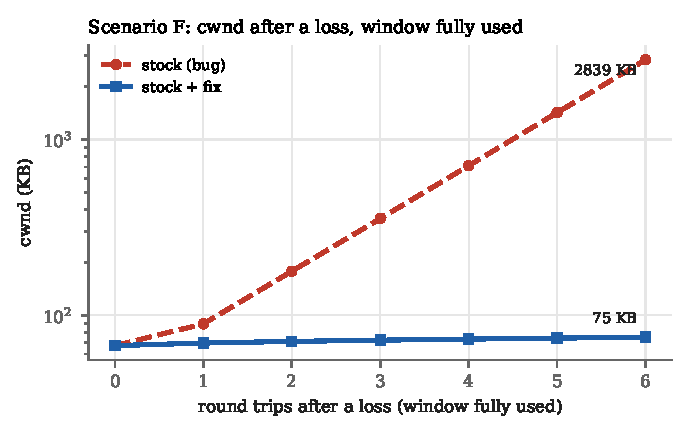
\includegraphics[width=0.6\textwidth]{figures/bug_harness.pdf}
  \caption{Scenario F, cwnd per round after the loss (log scale).}
\end{figure}

%======================================================================
\section{Evidence 5: effect on a real network path}

\paragraph{Isolation.} These runs use MsQuic \texttt{464c873c0} (31 August
2026, the base of our project), not today's \texttt{main}. Between the two,
\texttt{cubic.c} changed only in how the active path is looked up
(\texttt{Connection->Paths[0]} became \texttt{QuicPathGetActive(...)}, 12
places, plus line wrapping); the AIMD code and all window arithmetic are
identical. The
``upstream'' build is that commit's CUBIC. The ``fixed'' build is our ablation
source with every one of our rate-limited-sender changes compiled out by
macros, plus the two-line swap. We checked that this configuration is exactly
equivalent: in our deterministic harness (504 trace rows) it produces the same
trace as upstream plus the swap, and with the swap undone the same trace as
upstream, so the only behavioural difference between the two builds is the
swap. The direct-observation run below goes
one step further: its two builds are compiled from sources that differ
textually in the two lines only (\texttt{experiments/acc\_proof/S0\_vs\_S1.diff}).

\paragraph{Testbed.} Linux network namespaces with a \texttt{netem}
bottleneck (10--50\,Mbit/s, 41--81\,ms RTT, 100-packet drop-tail queue,
segmentation offloads off). A QUIC sender sends 3\,MB, then 6000\,B every
10\,ms, then 8\,MB. 10 runs per build and setting, build order rotated; medians,
two-sided permutation tests (20\,000 permutations).

\begin{table}[H]
\centering\footnotesize
\setlength{\tabcolsep}{4pt}
\begin{tabular}{@{}lcccccc@{}}
\toprule
 & \multicolumn{2}{c}{full-packet CA} & \multicolumn{2}{c}{cwnd at} & \multicolumn{2}{c}{lost after} \\
 & \multicolumn{2}{c}{increases} & \multicolumn{2}{c}{resume (KB)} & \multicolumn{2}{c}{resume (KB)} \\
\cmidrule(lr){2-3}\cmidrule(lr){4-5}\cmidrule(l){6-7}
Setting & upstream & fixed & upstream & fixed & upstream & fixed \\
\midrule
6\,s rate-limited, 10\,Mbit/s & 33\,\% & 1.0\,\% & 668 & 229 & 3413 & 82 \\
28\,s rate-limited, 10\,Mbit/s & 23\,\% & 0.7\,\% & 670 & 671 & 1094 & 1094 \\
6\,s, RTT 81\,ms & 25\,\% & 0.2\,\% & 762 & 232 & 2800 & 84 \\
10\,s, 50\,Mbit/s & 22\,\% & 0.4\,\% & 668 & 288 & 3002 & 140 \\
25\,Mbit/s + TCP flow & 11\,\% & 5.7\,\% & 128 & 88 & 106 & 47 \\
\bottomrule
\end{tabular}
\caption{Upstream vs.\ upstream + the two-line fix on a real (emulated) network
  path; medians of 10 runs. The signature of the bug (a congestion-avoidance
  increase of exactly one packet on a single ACK) drops from 11--33\,\% to
  0.2--6\,\% of increases ($p \le 0.012$ in every setting). Where the bug has
  time to act (6--10\,s) it inflates the window 2.3--3.3$\times$ and the loss
  after resumption 21--42$\times$ ($p < 0.004$). After 28\,s plain CUBIC
  reaches the same limit on its own, so the window and loss are equal
  ($p > 0.6$): the fix does not change anything it should not.}
\end{table}

\paragraph{Direct observation of the accumulator.}
We repeated two settings with builds that log \aw\ and \acc\ on every ACK.
The two sources differ textually only in the swap
(\texttt{experiments/acc\_proof/S0\_vs\_S1.diff}) and contain none of our
rate-limited-sender code. Both are upstream \texttt{464c873c0}'s
\texttt{cubic.c} plus a trace logger, compiled in the same tree. That tree
also holds our test client (\texttt{sample.c}) and one extra field in
\texttt{cubic.h} that neither source uses; both are the same for the two
builds. Since \acc\ only ever holds acknowledged bytes
(at most a few hundred KB here), a value $\ge 2^{31}$ can only be a wrap; no
model or threshold tuning is involved.

\begin{table}[H]
\centering\footnotesize
\setlength{\tabcolsep}{2.6pt}
\begin{tabular}{@{}llcccccc@{}}
\toprule
Setting & Build & runs with & wrap events & full-packet & cwnd at & lost after & max \acc \\
 & & a wrap & (median) & CA incr. & resume (KB) & resume (KB) & (bytes) \\
\midrule
6\,s RL, 10\,Mbit/s & upstream & 10/10 & 22 & 32\,\% & 668 & 3351 & $4.29\times10^{9}$ \\
 & fixed & 0/10 & 0 & 0.9\,\% & 218 & 72 & 163\,285 \\
25\,Mbit/s + TCP & upstream & 10/10 & 84 & 16\,\% & 146 & 765 & $4.29\times10^{9}$ \\
 & fixed & 0/10 & 0 & 3.6\,\% & 80 & 32 & 129\,874 \\
\bottomrule
\end{tabular}
\caption{Accumulator logged on every ACK, 10 runs per build and setting
  (medians; RL = rate-limited; ``max \acc'' is the largest value seen in any
  run of the setting). Upstream vs.\
  fixed: $p = 0.0001$ for cwnd, loss and full-packet share in the 6\,s
  setting; $p = 0.016$, $0.008$ and $0.004$ in the TCP setting. The 6\,s row
  reproduces the four-build campaign above (668 vs.\ 229\,KB, 3413 vs.\
  82\,KB).}
\label{tab:accnet}
\end{table}

Across all ACKs the upstream build processed 90\,764 ACKs, and after 27\,940
of them \acc\ held a wrapped value; the fixed build processed 92\,400 ACKs and
never did. In 522 fixed-build ACKs \acc\ was larger than \aw\ without being
wrapped. We checked each one: all 28 such stretches start exactly at a
congestion event, where MsQuic lowers \aw\ but keeps \acc, and \acc\ stays
unchanged through recovery until the next growing ACK subtracts the window
normally. This is upstream behaviour unrelated to the swap.
Figure~\ref{fig:accnet} shows one representative run per build (the run with
the median number of wrap events): the upstream accumulator sits at
$\approx 2^{32}$ or jumps there dozens of times, and each time cwnd climbs by
one packet per ACK; the fixed accumulator never exceeds $1.7\times10^5$.

\begin{figure}[H]
\centering
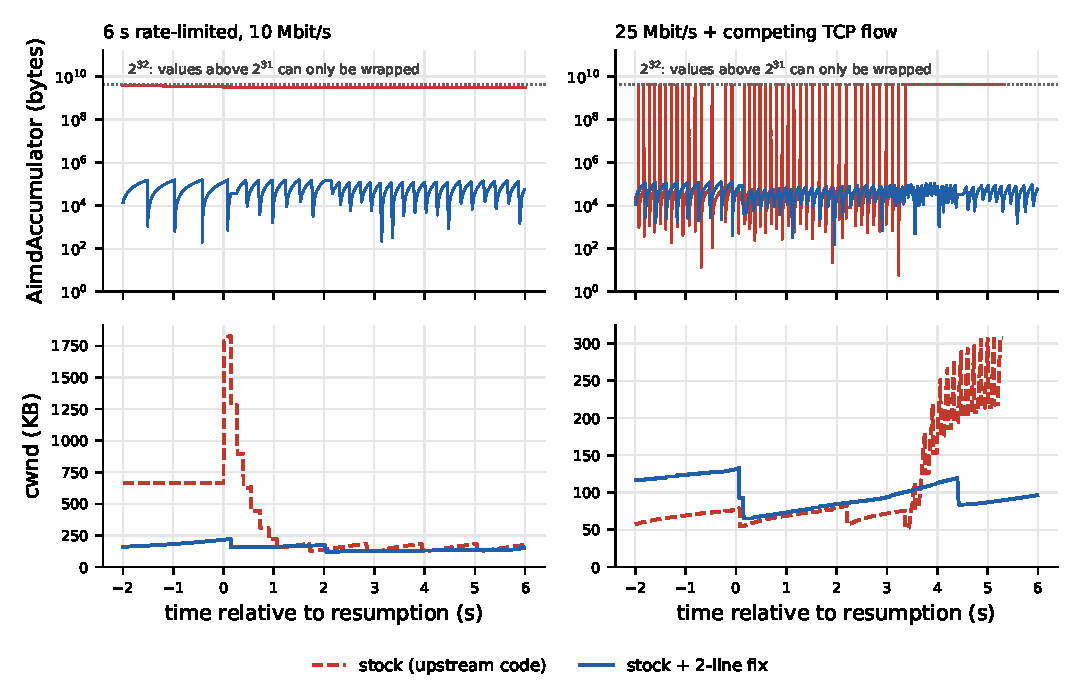
\includegraphics[width=\linewidth]{figures/acc_network.pdf}
\caption{\acc\ (log scale, top) and cwnd (bottom) on every ACK around the
  resumption of bulk sending, upstream vs.\ upstream + the two-line fix.
  Left: 6\,s rate-limited at 10\,Mbit/s (the upstream accumulator wrapped
  during the rate-limited phase and stays wrapped, so cwnd is already 668\,KB
  at resumption). Right: 25\,Mbit/s with a competing TCP flow.}
\label{fig:accnet}
\end{figure}

\paragraph{Plain bulk transfers.}\label{sec:bulk}
Our largest effects come after a rate-limited phase, the scenario of our
project. To see whether the bug matters without one, we ran the same two
logging builds on single bulk transfers with no rate-limited phase (10 runs
per build and setting, build order rotated): 30\,MB at 10\,Mbit/s with 40 and
80\,ms RTT, 100\,MB at 50\,Mbit/s, and 60\,MB at 25\,Mbit/s shared with a
TCP CUBIC flow (\texttt{sudo experiments/run\_campaign.sh bulk}).

The wrap happened in all 40 upstream runs and in
none of the 40 fixed runs (30--515 wraps per upstream run), but in most runs
it did no harm. A wrapped
accumulator is undone by the next ACK whenever that ACK adds more than the
shortfall, which is always less than one packet: the \texttt{uint32} addition
wraps it back to a small value. With the usual ACK of two packets this always
happens. The wrap \emph{persists} only if the next ACK adds less than the
shortfall. That happened in 10 of the 40 upstream runs, and in all 10 the
cause was the same: a single-packet ACK (1472\,B) while \aw\ was below
\texttt{WindowPrior}, where the code counts only half of each ACK (736\,B).
From then on every ACK subtracts the growing window from a value near
$2^{32}$, so the accumulator stays wrapped for thousands of ACKs (1\,248 to
20\,464 here), usually until the end of the transfer.

\begin{table}[H]
\centering\footnotesize
\setlength{\tabcolsep}{3.5pt}
\begin{tabular}{@{}lcccc@{}}
\toprule
 & \multicolumn{2}{c}{upstream} & fixed & runs with persistent \\
\cmidrule(lr){2-3}\cmidrule(lr){4-4}
Setting & wrap persisted & wrap undone & & wrap (upstream vs.\ fixed) \\
\midrule
10\,Mbit/s, 40\,ms & --- & 164--180 (10 runs) & 171--182 & 0/10 vs.\ 0/10 \\
10\,Mbit/s, 80\,ms & \textbf{1\,056--3\,241} (3) & 192--202 (7) & 194--203 & 3/10 vs.\ 0/10 \\
50\,Mbit/s, 40\,ms & \textbf{582--6\,244} (2) & 114--131 (8) & 114--123 & 2/10 vs.\ 0/10 \\
25\,Mbit/s + TCP & \textbf{845--10\,935} (5) & 65--98 (5) & 73--100 & 5/10 vs.\ 0/10 \\
\bottomrule
\end{tabular}
\caption{Lost packets per bulk transfer (range over runs; number of runs in
  brackets). Last column: runs in which the wrap persisted for more than 100
  ACKs, upstream vs.\ fixed (10/40 vs.\ 0/40 overall, Fisher exact test
  $p = 0.001$). Upstream runs whose wraps were all undone are
  indistinguishable from the fixed build in every metric we measured; runs
  with a persistent wrap lose 5--130$\times$ more packets than the fixed
  build's median.}
\label{tab:bulk}
\end{table}

\begin{figure}[H]
\centering
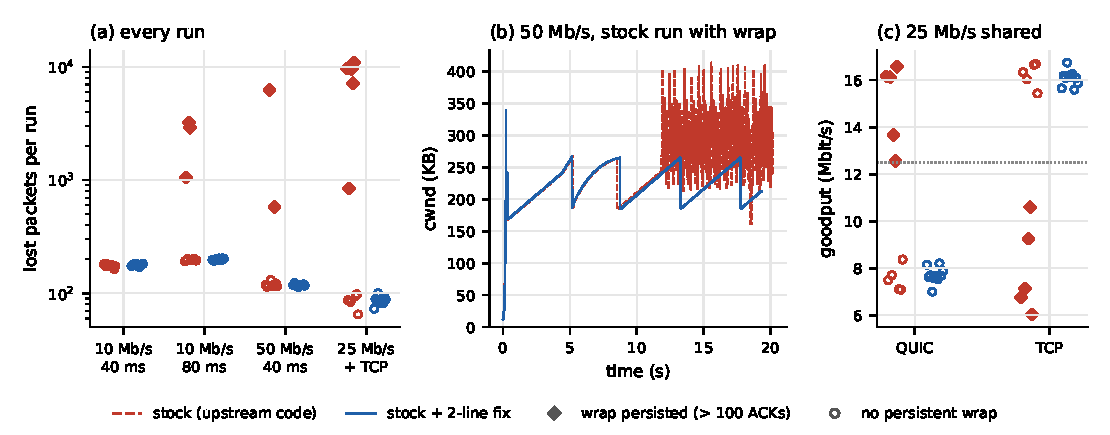
\includegraphics[width=\linewidth]{figures/bulk_network.pdf}
\caption{Plain bulk transfers. (a) Lost packets in every run; filled diamonds
  are upstream runs in which the wrap persisted. (b) cwnd at 50\,Mbit/s in the
  upstream run with the longest wrap and a typical fixed run: once the wrap
  persists (at about 12\,s), cwnd grows by one packet per ACK until a loss,
  over and over. (c) Goodput of the QUIC transfer and the competing TCP flow
  at 25\,Mbit/s, per run; the dotted line is an equal share.}
\label{fig:bulk}
\end{figure}

Without competition the link is full either way, so completion time does not
change (medians within 0.01\,s); what a persistent wrap adds is
self-inflicted loss and queue overflow at the bottleneck. With a competing TCP
flow it also changes the split of the link. In the five upstream runs with a
persistent wrap the QUIC transfer got a median 16.1\,Mbit/s and TCP
7.1\,Mbit/s; in the fixed runs QUIC got 7.7 and TCP 16.1\,Mbit/s. We note
honestly that with the fix the QUIC flow gets \emph{less} than half of the
link against Linux TCP CUBIC. The bug happens to push it the other way, but
by making it far more aggressive than RFC~9438 allows (one packet per ACK
instead of 0.5 packet per RTT), not by correcting whatever causes that gap,
which we have not investigated.

%======================================================================
\section{Evidence 6: nothing else changes}

\begin{table}[H]
\centering\small
\begin{tabular}{@{}lcccc@{}}
\toprule
Upstream \texttt{main} (\texttt{3c9ec01c1}) & Tests & Passed & Skipped & Failed \\
\midrule
unmodified & 563 & 559 & 4 & 0 \\
+ fix, 2 new tests, 2 updated expectations & 565 & 561 & 4 & 0 \\
\bottomrule
\end{tabular}
\caption{MsQuic's full core test suite (\texttt{msquiccoretest}, all 39 suites).}
\end{table}
The only difference is the two new tests. The fix touches only the branch
taken when the accumulator crosses the window; whenever it crosses by a full
packet or more, the old and new order give the same \aw\ and differ only in the
accumulator's remainder (which the old order understated by one packet).

\paragraph{The two updated expectations.} Two upstream tests hard-code the old
order: \texttt{AIMD\_\allowbreak{}Accumulator\allowbreak{}Triggers\allowbreak{}Window\allowbreak{}Growth} expects
$1432 - (100 + 1232) = 100$, i.e.\ ``subtract the grown window'', after
choosing its ACK size ``to avoid unsigned underflow''; and
\texttt{AIMD\_\allowbreak{}Sequential\allowbreak{}Linear\allowbreak{}Convergence} computes its expected values in the
old order. Both now expect ``subtract the window that was crossed, then grow''
(the accumulator keeps $1432 - 100 = 1332$ bytes). No other test changed.

%======================================================================
\section{How we ruled out mistakes on our side}

\begin{itemize}
  \item \textbf{Our patch is not involved.} Evidence 1, 2 and 6 use a fresh
        checkout of upstream \texttt{main} with nothing of ours except the two
        tests. In Evidence 5 our patch is compiled out (four-build campaign)
        or absent (direct-observation run).
  \item \textbf{Exactly two lines.} In Evidence 1, 2, 4 and the
        direct-observation run the compared sources differ textually only in
        the swap; the diffs are in \texttt{experiments/acc\_proof/} and the
        source hashes are recorded.
  \item \textbf{Independent tools.} The wrap is reported by gdb reading
        upstream's variables, and by MsQuic's own test runner; our analysis
        scripts are not needed for Evidence 1--4.
  \item \textbf{Run by a third party.} Evidence 1, 2 and 6 were re-run on
        GitHub's servers by a GitHub Actions workflow
        (\texttt{.github/workflows/aimd-proof.yml}). It clones
        \texttt{microsoft/msquic} directly from GitHub, at \texttt{3c9ec01c1}
        and at the then-current \texttt{main}, and checks every expected
        outcome itself: both reproducers fail, gdb catches the wrap in
        upstream's own tests, the change to \texttt{cubic.c} is exactly one
        moved line, and with it the reproducers, all CUBIC tests and the full
        core suite pass. Both jobs succeeded on 12 November 2026; the log and
        raw outputs are hosted by GitHub, not by us:
        \url{https://github.com/Abhirams144/msquic-rate_limited_sender_increase/actions/runs/43286985783}.
  \item \textbf{No inference needed.} In the direct-observation run the wrap
        is read from the logged variable itself ($\ge 2^{31}$), not inferred
        from cwnd: 20/20 upstream runs vs.\ 0/20 fixed runs.
  \item \textbf{Natural inputs.} The behavioural reproducer and the network
        runs set no internal state; the bug appears on its own.
  \item \textbf{When the bug is harmless.} A wrap is undone by the next ACK
        whenever that ACK adds more than the shortfall (less than one
        packet), which is the normal case in steady bulk transfer. It
        persists after a single-packet ACK while \acc\ counts half of each
        ACK (below \texttt{WindowPrior}), which is common when sending is
        rate-limited or another flow shares the queue, and happened in
        10 of 40 plain bulk transfers (Section~\ref{sec:bulk}). The effect
        is therefore all-or-nothing per occurrence, not a small bias.
\end{itemize}

%======================================================================
\section{Reproducing everything}
\label{sec:repro}

\begin{lstlisting}
# 1. upstream main + the two tests, before and after the fix
git -C msquic worktree add --detach ../upstream-main 3c9ec01c1
cd upstream-main && git submodule update --init submodules/{clog,quictls,googletest}
cmake -B build-test -DQUIC_BUILD_TEST=ON -DQUIC_TLS_LIB=quictls -DCMAKE_BUILD_TYPE=Debug
cat ../experiments/acc_proof/reproducer_tests.cpp >> src/core/unittest/CubicTest.cpp
cmake --build build-test --target msquiccoretest
build-test/bin/Debug/msquiccoretest --gtest_filter='CubicTest.AIMD_*'      # fails
git apply ../experiments/acc_proof/fix_on_upstream_main.diff               # the 2 lines
# 2. catch the wrap with gdb (on the unfixed build)
gdb -batch -x ../experiments/acc_proof/catch_wrap.gdb \
    --args build-test/bin/Debug/msquiccoretest --gtest_filter='CubicTest.*'
# 3. full core suite: build-test/bin/Debug/msquiccoretest --gtest_brief=1
# 4. network: experiments/acc_proof/build_acc.sh; sudo experiments/run_campaign.sh acc
#             python3 experiments/acc_proof/analyze_acc.py
#    bulk:    sudo experiments/run_campaign.sh bulk
#             python3 experiments/acc_proof/analyze_bulk.py
\end{lstlisting}

\end{document}
